%% Esqueleto do paper (ADR 0011). Template oficial do CBSoft 2026 (acmart, sigconf).
%% Blocos \topicos{...} em cinza = o que a seção deve dizer, com os números. O Caio troca por prosa.
%% Para a submissão anônima do SBES, trocar para \documentclass[sigconf,anonymous]{acmart}.
\documentclass[sigconf]{acmart}
\settopmatter{printacmref=false}
\renewcommand\footnotetextcopyrightpermission[1]{}
\setcopyright{none}
\acmConference[SBES 2026]{40th Brazilian Symposium on Software Engineering}{September 8--12, 2026}{São Paulo, SP, Brazil}
\AtBeginDocument{\providecommand\BibTeX{{Bib\TeX}}}

\usepackage[portuguese]{babel}
\usepackage{xcolor}
\newcommand{\SaposN}{29}
\newcommand{\SaposKappa}{[$\kappa$ a medir]}
\newcommand{\SaposAmploN}{67}

\AtBeginDocument{\renewcommand{\acksname}{Agradecimentos}}
\newcommand{\topicos}[1]{{\color{gray}\begin{itemize}\setlength\itemsep{0pt}#1\end{itemize}}}

\begin{document}

\title{Estruturar a issue ajuda o agente? Reescrita com Agent Skills e com critérios da literatura na resolução automática de issues}

\author{Caio Paranhos}
\affiliation{
  \institution{Instituto de Computação, Universidade Federal Fluminense}
  \city{Niterói}
  \country{Brasil}
}

\renewcommand{\shortauthors}{Paranhos}

\begin{abstract}
\textcolor{gray}{[Um parágrafo só. Contexto: agentes de IA resolvem issues sozinhos. Pergunta: reescrever a issue de forma estruturada (skill Spec-Driven Development; critérios de Bettenburg/Heck) muda eficácia, custo e qualidade do patch? Método: 3 grupos (skill, original, literatura), Sonnet 5.5 resolve, testes fail-to-pass como oráculo, SWE-bench Lite (296 issues) e SAPOS (\SaposN\ issues reais, recentes). Resultado: nenhuma diferença detectável na taxa de resolução; a skill custa \textasciitilde40\% mais tokens e leva o agente a mexer mais em arquivos errados; SWE-bench mostra sinais fortes de contaminação. Conclusão em uma frase.]}
\end{abstract}

\keywords{agentes de IA, issues, Agent Skills, SWE-bench, qualidade de relato de defeito}

\maketitle

\section{Introdução}
\topicos{
\item Issue é o centro da coordenação; descrição ruim atrasa a correção \cite{bettenburg2008,zimmermann2010}; LLMs já são usados para melhorar relatos \cite{acharya2025}.
\item Hoje o leitor da issue também é um agente autônomo (Claude, Devin, Cursor) que abre PRs sozinho.
\item Agent Skills prometem estruturar o trabalho do agente; a skill Spec-Driven Development \cite{osmani2024skills} transforma um pedido em especificação.
\item Pergunta: a premissa ``issue bem estruturada resolve mais rápido'' vale quando quem lê é um agente?
\item RQ1 eficácia (resolve mais?), RQ2 eficiência e custo (tokens, tempo), RQ3 qualidade do patch.
\item Contribuições: (i) experimento com 3 grupos em 296 issues do SWE-bench Lite; (ii) evidência de contaminação do SWE-bench (vazamento na reescrita e memória do resolvedor); (iii) réplica em \SaposN\ issues reais e recentes do SAPOS, sistema open source da UFF.
}

\section{Trabalhos relacionados}
\topicos{
\item Qualidade de relato: Bettenburg et al.~\cite{bettenburg2008} (passos para reproduzir, observado/esperado, stack trace, caso de teste); Heck e Zaidman~\cite{heck2017} (QC1: descrição, justificativa, cenário, solução).
\item Tipo de issue: Herzig et al.~\cite{herzig2013} (bug $\neq$ feature em \textasciitilde1/3 dos casos); LLM como classificador \cite{colavito2024}.
\item Benchmarks: SWE-bench \cite{jimenez2024swebench}; contaminação e benchmarks vivos: SWE-rebench \cite{badertdinov2025swerebench}, SWE-bench-Live \cite{zhang2025swebenchlive}.
\item Lacuna: ninguém mediu o efeito de \emph{reescrever} a issue (com skill ou com critério da literatura) sobre o agente que resolve.
}

\section{Metodologia}
\begin{figure}[t]
\centering
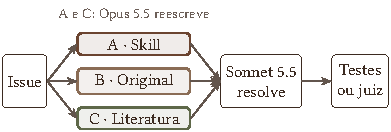
\includegraphics[width=\columnwidth]{overview.pdf}
\caption{Visão geral do experimento: a mesma issue em três versões, resolvida pelo agente e avaliada por testes ou juiz LLM.}
\label{fig:metodologia}
\end{figure}

\topicos{
\item Grupos (Fig.~\ref{fig:metodologia}): A = Opus 5.5 reescreve com a skill (só a 1ª etapa, especificação, porque a skill pede aprovação humana a cada etapa); B = texto original (baseline); C = Opus 5.5 reescreve com os itens da literatura do tipo da issue. O Gerador vê só o texto da issue.
\item Classificação bug/feature: skill de classificação com as regras da Tabela III de Herzig et al.~\cite{herzig2013} no molde de Colavito et al.~\cite{colavito2024}, zero-shot; $\kappa$ 0,714 contra anotação manual em outro conjunto (issues abertas por agentes); \SaposKappa\ contra anotação cega do autor no SAPOS.
\item Resolvedor: Sonnet 5.5, sem humano, dentro do container da issue, sem busca na web, 1 execução por issue e grupo, limite de 60 min.
\item Oráculo: testes FAIL\_TO\_PASS e PASS\_TO\_PASS, como no SWE-bench.
\item Corpus 1: SWE-bench Lite \cite{jimenez2024swebench}, 300 issues; 4 excluídas (nem o fix oficial passa no ambiente); 229 bug, 40 feature, 27 nenhum dos dois.
\item Corpus 2: SAPOS (sistema da UFF, Ruby on Rails): 432 issues fechadas, 340 com correção em código, 67 com commit base no ambiente atual (Ruby 3.2/3.4; o resto exige Rails 3--6); nível estrito: as \SaposN\ com $\geq$1 teste FAIL\_TO\_PASS. Reescrita em português; instruções de agente do repositório (\texttt{AGENTS.md}) removidas do container.
\item Dois níveis no SAPOS: estrito (testes, como no SWE-bench) e amplo (juiz LLM, Opus 5.5, cego quanto ao grupo, calibrado contra os testes do nível estrito; uma única revisão da régua, $\kappa$ medido numa metade não usada para ajuste).
\item Medidas: resolvida (RQ1); tokens, tempo, custo estimado a preço de tabela da API (RQ2); arquivos iguais aos do fix oficial, testes quebrados, tamanho do patch (RQ3).
}

\section{Resultados}
\begin{table}[t]
\caption{SWE-bench Lite: as mesmas 269 issues bug/feature nos três grupos.}
\label{tab:swebench}
\small
\begin{tabular}{lrrr}
\toprule
 & A (skill) & B (original) & C (literatura) \\
\midrule
Resolvidas & 191 (71\%) & 189 (70\%) & 188 (70\%) \\
Tokens de entrada (mediana) & 104.201 & 74.428 & 77.957 \\
Custo estimado, US\$ (mediana) & 0,067 & 0,049 & 0,052 \\
Tempo, s (mediana) & 17 & 14 & 14 \\
Mesmos arquivos do fix oficial & 227 (84\%) & 249 (93\%) & 251 (93\%) \\
Quebra teste que passava & 13 (5\%) & 11 (4\%) & 7 (3\%) \\
\bottomrule
\end{tabular}
\end{table}

\begin{table}[t]
\caption{SAPOS: as mesmas 20 issues nos três grupos.}
\label{tab:sapos}
\small
\begin{tabular}{lrrr}
\toprule
 & A (skill) & B (original) & C (literatura) \\
\midrule
Resolvidas & 4 (20\%) & 4 (20\%) & 4 (20\%) \\
Tokens de entrada (mediana) & 116.635 & 105.230 & 112.617 \\
Custo estimado, US\$ (mediana) & 0,099 & 0,080 & 0,069 \\
Tempo, s (mediana) & 23 & 20 & 17 \\
Mesmos arquivos do fix oficial & 5 (25\%) & 5 (25\%) & 8 (40\%) \\
Quebra teste que passava & 2 (10\%) & 2 (10\%) & 2 (10\%) \\
\bottomrule
\end{tabular}
\end{table}

\begin{table}[t]
\caption{SAPOS, nível amplo: resolvidas segundo o juiz LLM ($\kappa$ 0,76 contra os testes no nível estrito).}
\label{tab:sapos-amplo}
\small
\begin{tabular}{lrrr}
\toprule
 & A (skill) & B (original) & C (literatura) \\
\midrule
Todas (67) & 10 (15\%) & 10 (15\%) & -- \\
Bug/feature (43) & 6 (14\%) & 5 (12\%) & 4 (9\%) \\
\bottomrule
\end{tabular}
\end{table}

\topicos{
\item SWE-bench (Tab.~\ref{tab:swebench}): A, B e C resolvem quase o mesmo (diferenças de 1 a 4 issues; McNemar A$\times$B 22 vs.\ 20, $p=0{,}88$).
\item A custa mais: mediana de 104 mil tokens de entrada contra 74 mil (B) e 78 mil (C).
\item A acerta menos o lugar da correção: mesmos arquivos do fix oficial em 84\% contra 93\% (B e C).
\item SAPOS, nível estrito (Tab.~\ref{tab:sapos}): 29 tarefas com teste que falha antes da correção (de 48 com teste no ambiente atual); 20 bug/feature com os três grupos. Resolvidas: 4 de 20 (20\%) em A, B e C; nas 29, A 4 e B 4 (14\%). Três issues resolvidas pelos três grupos; uma troca (1$\times$1).
\item SAPOS, nível amplo (Tab.~\ref{tab:sapos-amplo}): 67 issues com correção em código e ambiente atual, julgadas por um juiz LLM calibrado nos testes do nível estrito ($\kappa$ 0,76; 0,90 na metade de teste). A 15\%, B 15\%; nas 43 bug/feature, A 14\%, B 12\%, C 9\%.
\item Queda de \textasciitilde70\% (SWE-bench) para 14--20\% (SAPOS) com o mesmo agente, nos dois níveis.
\item Custo no SAPOS: custo estimado maior em A (US\$ 0,10 contra 0,08 em B); A deixa o patch vazio em 7 de 29 (B: 4; C: 0 de 20).
\item Vazamento quase some no SAPOS: reescrita cita arquivo do fix ausente na issue em 1 de 27 (A) e 0 de 18 (C), contra 46 e 5 de 269 no SWE-bench.
}

\section{Discussão e ameaças à validade}
\topicos{
\item Contaminação do SWE-bench: a reescrita do grupo A cita arquivo do fix oficial ausente na issue em 46 de 269 casos (C: 5); 74 de 269 issues resolvidas em até 5 passos sem a issue citar o arquivo; exemplo pytest-5221 (busca direta por \texttt{\_showfixtures\_main}, ``Upstream format'').
\item Por que o SAPOS: projeto pequeno, issues posteriores ao corte de treino. Ameaça própria: correções de 2026 coescritas pelo Claude (mesma família do resolvedor) e issues longas, já estruturadas.
\item Empate exato no SAPOS (4/4/4) não é o mesmo conjunto: 3 issues fáceis resolvidas pelos três grupos (na \#648, patch idêntico) e uma troca (\#624 só em A; \#680 em B e C). Issues do SAPOS já são detalhadas (mediana de 1.828 caracteres contra 1.070; 56\% citam o arquivo a corrigir contra 46\%): pouco espaço para a reescrita.
\item Molde da skill é de especificação de projeto, não de relato de defeito; pode inventar requisitos (exemplo pytest-7168).
\item Uma execução por issue: o agente não é determinístico.
\item Classificação validada em outra população (issues de agentes).
}

\section{Conclusão}
\topicos{
\item Reescrever a issue não aumentou a taxa de resolução em nenhum dos dois corpora; a skill genérica aumentou o custo; o molde da literatura ficou neutro e vazou menos.
\item Fora do benchmark contaminado, o mesmo agente resolve 14--20\% em vez de \textasciitilde70\%: o SWE-bench superestima a capacidade em issues novas.
\item Trabalhos futuros: repetições por issue, benchmarks posteriores ao corte de treino \cite{badertdinov2025swerebench,zhang2025swebenchlive}, issues escritas por humanos versus por agentes.
}

\section*{Disponibilidade de Artefatos}
\topicos{
\item Scripts (coleta, validação das tarefas do SAPOS, execução dos grupos, medidas), prompts, textos gerados pelos grupos A e C, patches e relatórios de avaliação: repositório anônimo (\url{https://anonymous.4open.science/}) na submissão; público após aceite.
\item Dados de terceiros: SWE-bench Lite (Hugging Face) e SAPOS (GitHub, gems-uff/sapos).
}

\begin{acks}
\topicos{
\item Uso de IA generativa (política do SBES): Claude Opus 5.5 (Anthropic) foi usado para escrever o código do experimento, executar as rodadas, gerar as tabelas e a Figura~\ref{fig:metodologia} e propor a estrutura deste artigo; o texto foi escrito pelo autor. Os modelos Claude Opus 5.5 e Sonnet 5.5 também são objeto do estudo (Gerador e Resolvedor).
}
\end{acks}

\bibliographystyle{ACM-Reference-Format}
\bibliography{refs}

\end{document}
